% ============================================================
% DIAGRAM: Backpropagation (1974/1986)
% ============================================================
% Caption: Figure 3.1: Multi-layer Perceptron with backpropagation.
%          (Adapted from Rumelhart, Hinton & Williams, 1986, p. 534)
% ============================================================

\documentclass[tikz,border=10pt]{standalone}
\usepackage{tikz}
\usepackage{amsmath}
\usepackage{amsfonts}

\usetikzlibrary{shapes,arrows,positioning,fit,calc,backgrounds}

\begin{document}

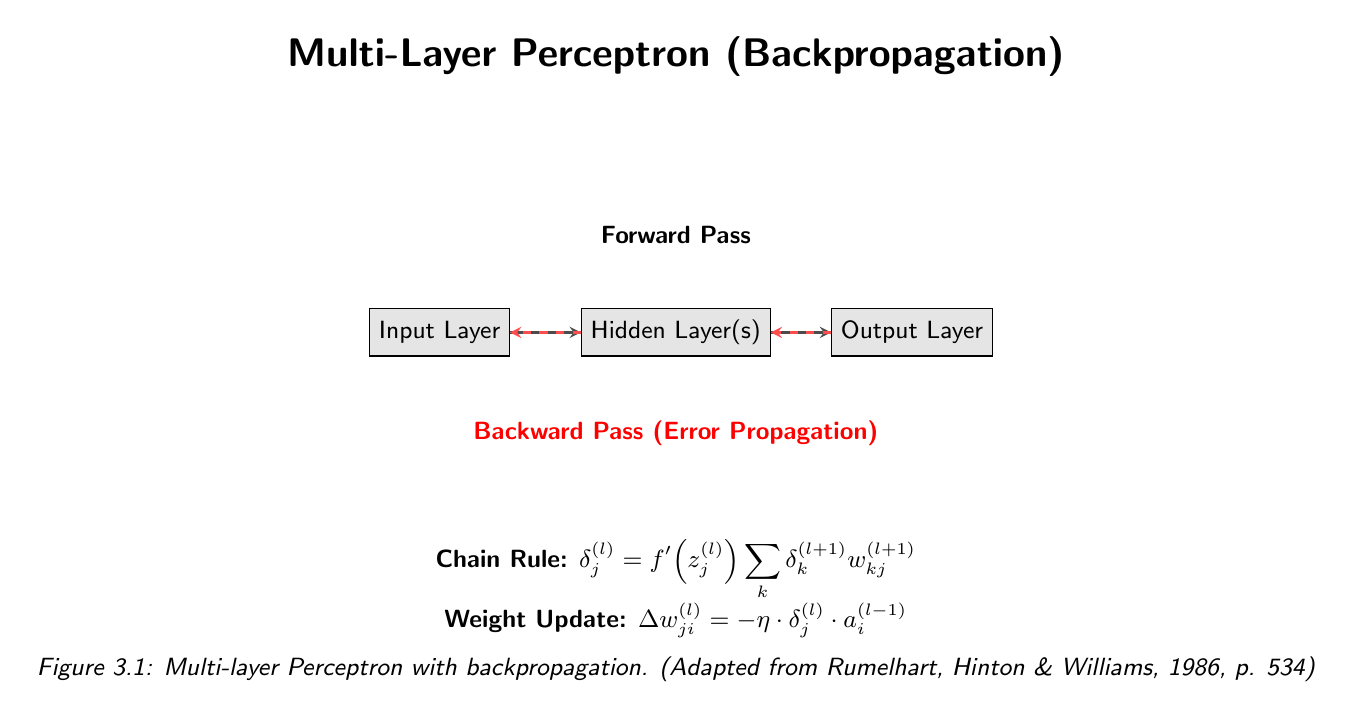
\begin{tikzpicture}[
    layer/.style={draw, rectangle, minimum width=1.2cm, minimum height=0.6cm, fill=gray!20, font=\sffamily\small},
    edge/.style={-stealth, thick, draw=black!70},
    redge/.style={-stealth, thick, draw=red!70, dashed},
    label/.style={font=\sffamily\small},
    title/.style={font=\sffamily\Large\bfseries},
    caption/.style={font=\sffamily\small\itshape},
]

\node[title] at (0, 3.5) {Multi-Layer Perceptron (Backpropagation)};

% Layers
\node[layer] (input) at (-3, 0) {Input Layer};
\node[layer] (hidden) at (0, 0) {Hidden Layer(s)};
\node[layer] (output) at (3, 0) {Output Layer};

% Forward pass (solid arrows)
\draw[edge] (input) -- (hidden);
\draw[edge] (hidden) -- (output);

% Backward pass (dashed red arrows)
\draw[redge] (output) -- (hidden);
\draw[redge] (hidden) -- (input);

% Labels
\node[above, font=\sffamily\small] at (0, 1) {\textbf{Forward Pass}};
\node[below, font=\sffamily\small, text=red] at (0, -1) {\textbf{Backward Pass (Error Propagation)}};

% Error
\node[align=center, font=\sffamily\small, anchor=north] at (0, -2.5) {
  \textbf{Chain Rule:} $\displaystyle \delta^{(l)}_j = f'\!\left(z^{(l)}_j\right) \sum_k \delta^{(l+1)}_k w^{(l+1)}_{kj}$ \\
  \textbf{Weight Update:} $\Delta w^{(l)}_{ji} = -\eta \cdot \delta^{(l)}_j \cdot a^{(l-1)}_i$
};

\node[caption, anchor=north] at (0, -4.0) {
  Figure 3.1: Multi-layer Perceptron with backpropagation. (Adapted from Rumelhart, Hinton \& Williams, 1986, p. 534)
};

\end{tikzpicture}
\end{document}
